\section{Backup modello di Ising 1D}

%----------------------------------------%
%		       Prima slide	     	     %
%	     Osservabili per N = 1000   	 %
%----------------------------------------%
\begin{frame}
    \frametitle{Osservabili per $N_s$ = 1000, h = 0.0}
    \framesubtitle{}

    \centering
    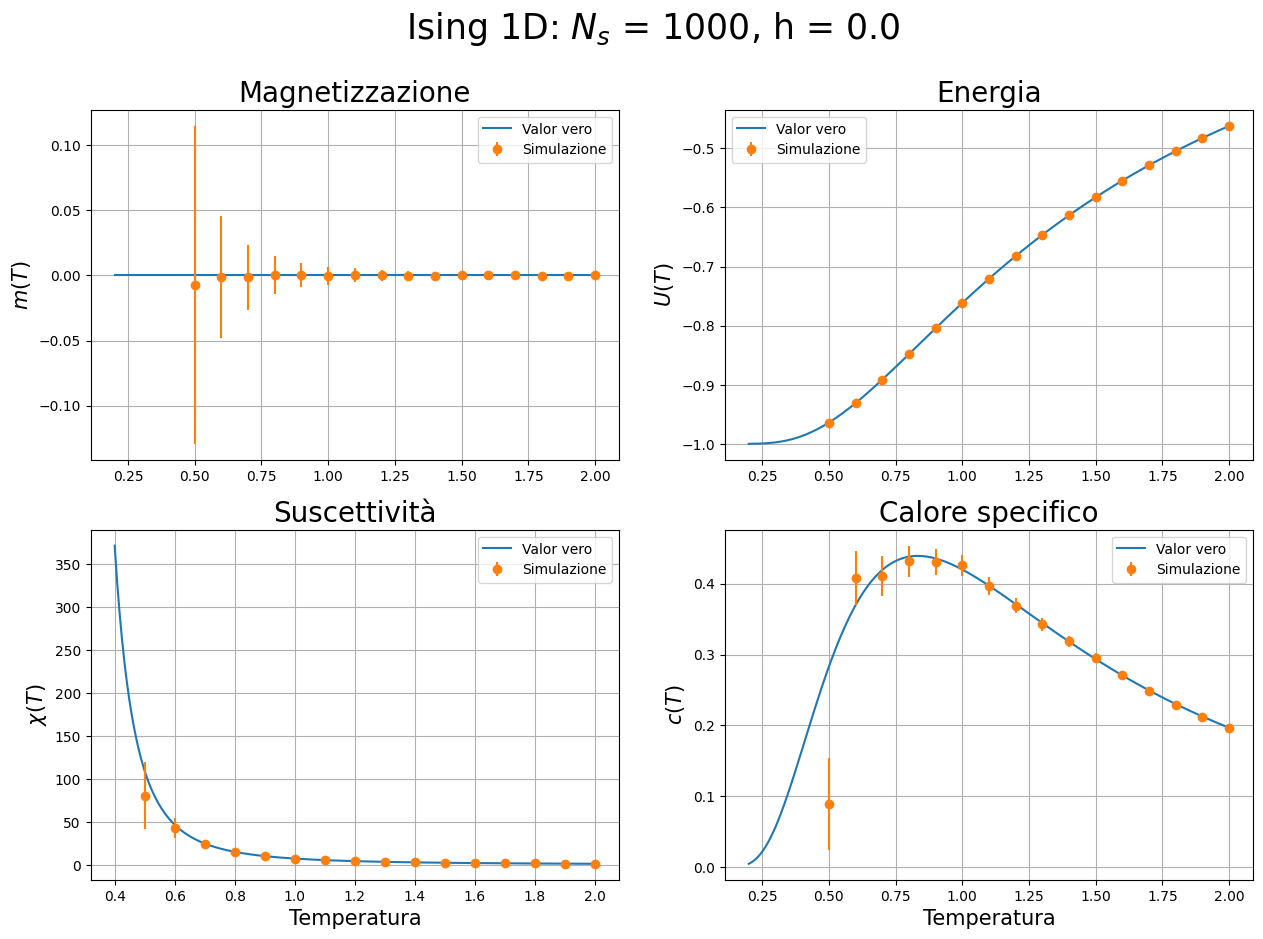
\includegraphics[width=0.65\textwidth]{Immagini/backupIsing1D/obs_1000_0.0.png}

\end{frame}



%----------------------------------------%
%		      Seconda slide	     	     %
% Differenza dal valor vero per N = 1000 %
%----------------------------------------%
\begin{frame}
    \frametitle{Differenza dal valor vero per $N_s$ = 1000, h = 0.0}
    \framesubtitle{}

    \centering
    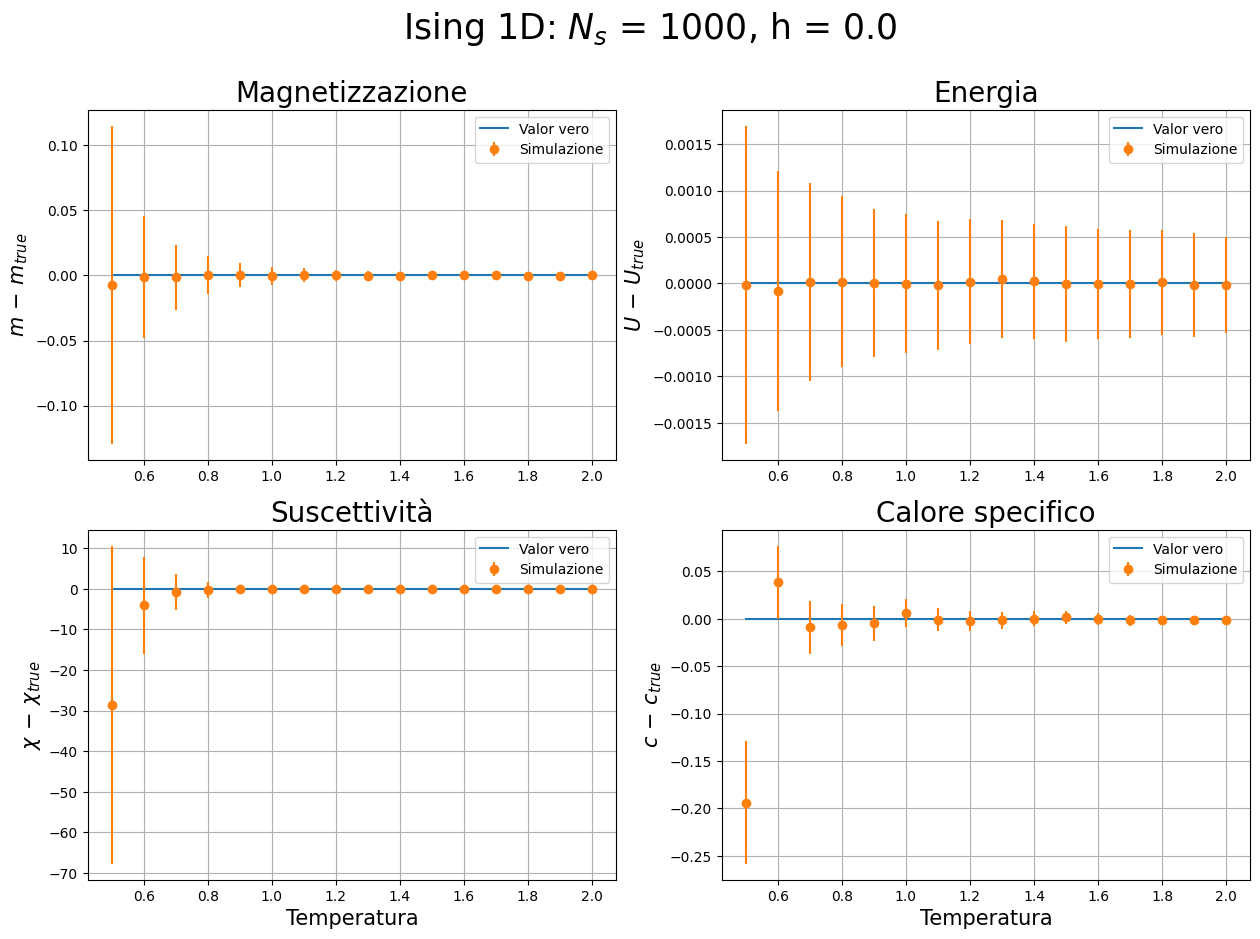
\includegraphics[width=0.65\textwidth]{Immagini/backupIsing1D/obs_1000_0.0_diff.png}

\end{frame}



%----------------------------------------%
%		       Terza slide	     	     %
%	     Osservabili per N = 3000   	 %
%----------------------------------------%
\begin{frame}
    \frametitle{Osservabili per $N_s$ = 3000, h = 0.0}
    \framesubtitle{}

    \centering
    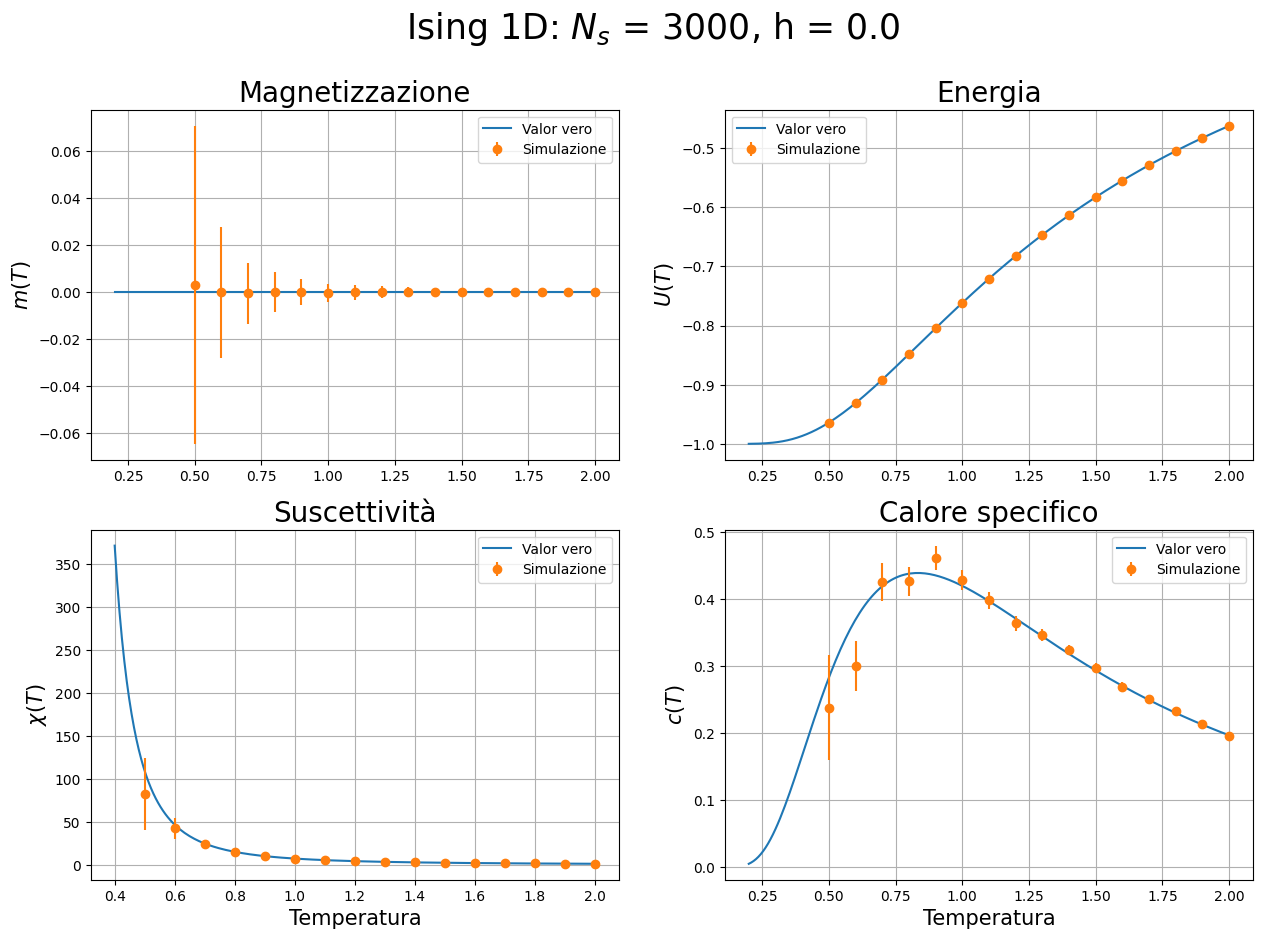
\includegraphics[width=0.65\textwidth]{Immagini/backupIsing1D/obs_3000_0.0.png}

\end{frame}



%----------------------------------------%
%		       Quarta slide	     	     %
% Differenza dal valor vero per N = 3000 %
%----------------------------------------%
\begin{frame}
    \frametitle{Differenza dal valor vero per $N_s$ = 3000, h = 0.0}
    \framesubtitle{}

    \centering
    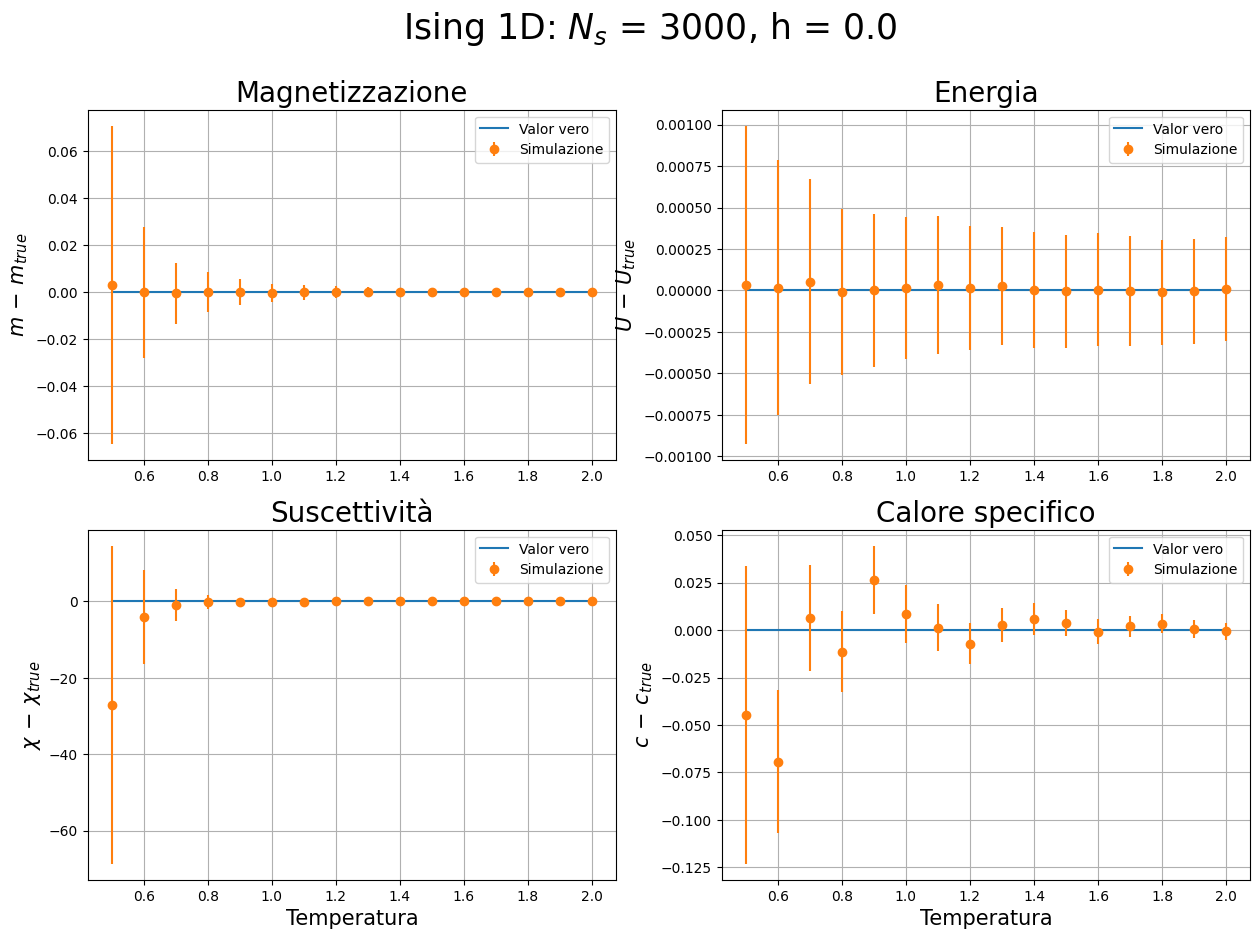
\includegraphics[width=0.65\textwidth]{Immagini/backupIsing1D/obs_3000_0.0_diff.png}

\end{frame}



%----------------------------------------%
%		       Quinta slide	     	     %
%	     Osservabili per N = 6000   	 %
%----------------------------------------%
\begin{frame}
    \frametitle{Osservabili per $N_s$ = 6000, h = 0.0}
    \framesubtitle{}

    \centering
    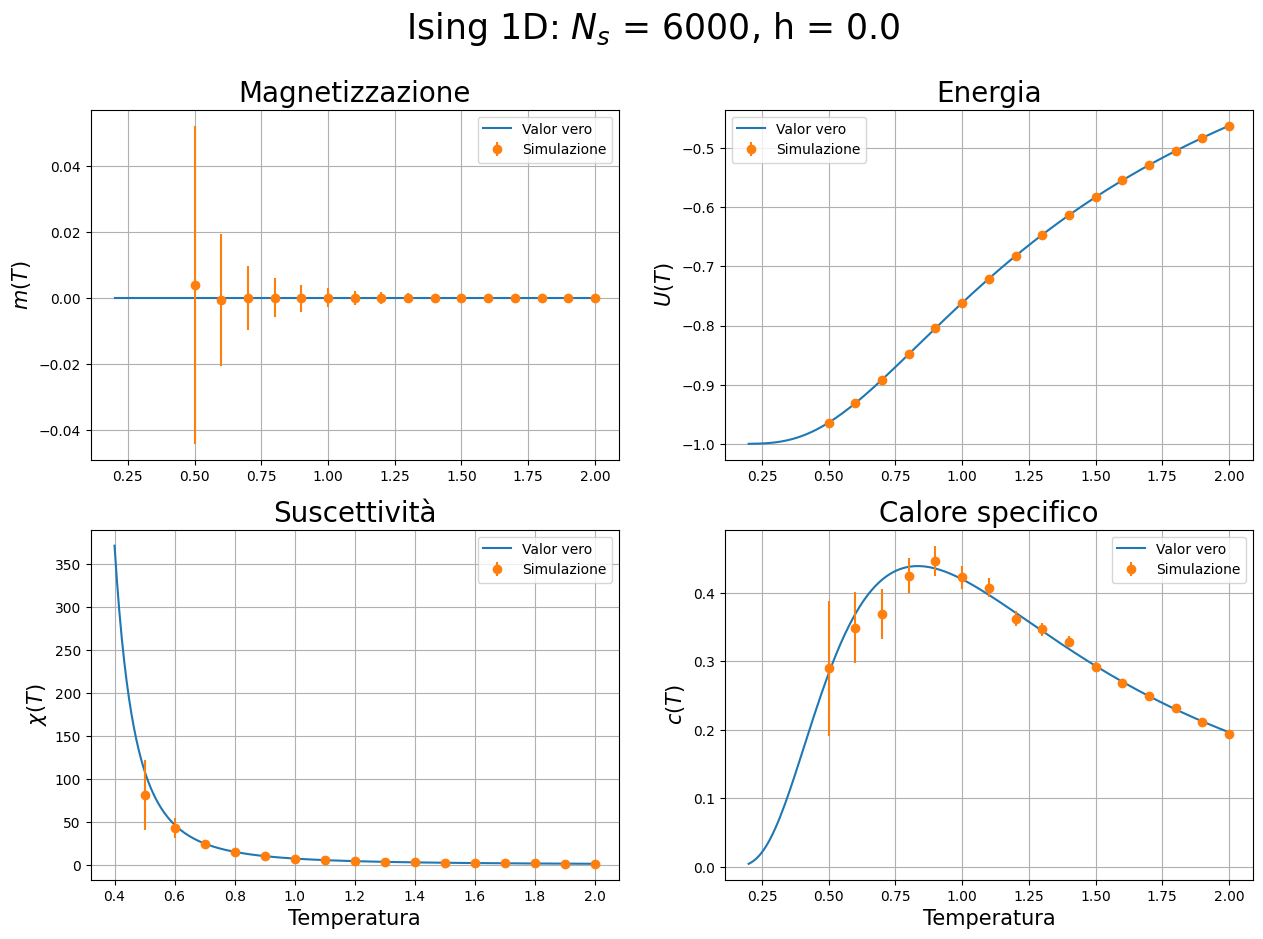
\includegraphics[width=0.65\textwidth]{Immagini/backupIsing1D/obs_6000_0.0.png}

\end{frame}



%----------------------------------------%
%		       Sesta slide	     	     %
% Differenza dal valor vero per N = 6000 %
%----------------------------------------%
\begin{frame}
    \frametitle{Differenza dal valor vero per $N_s$ = 6000, h = 0.0}
    \framesubtitle{}

    \centering
    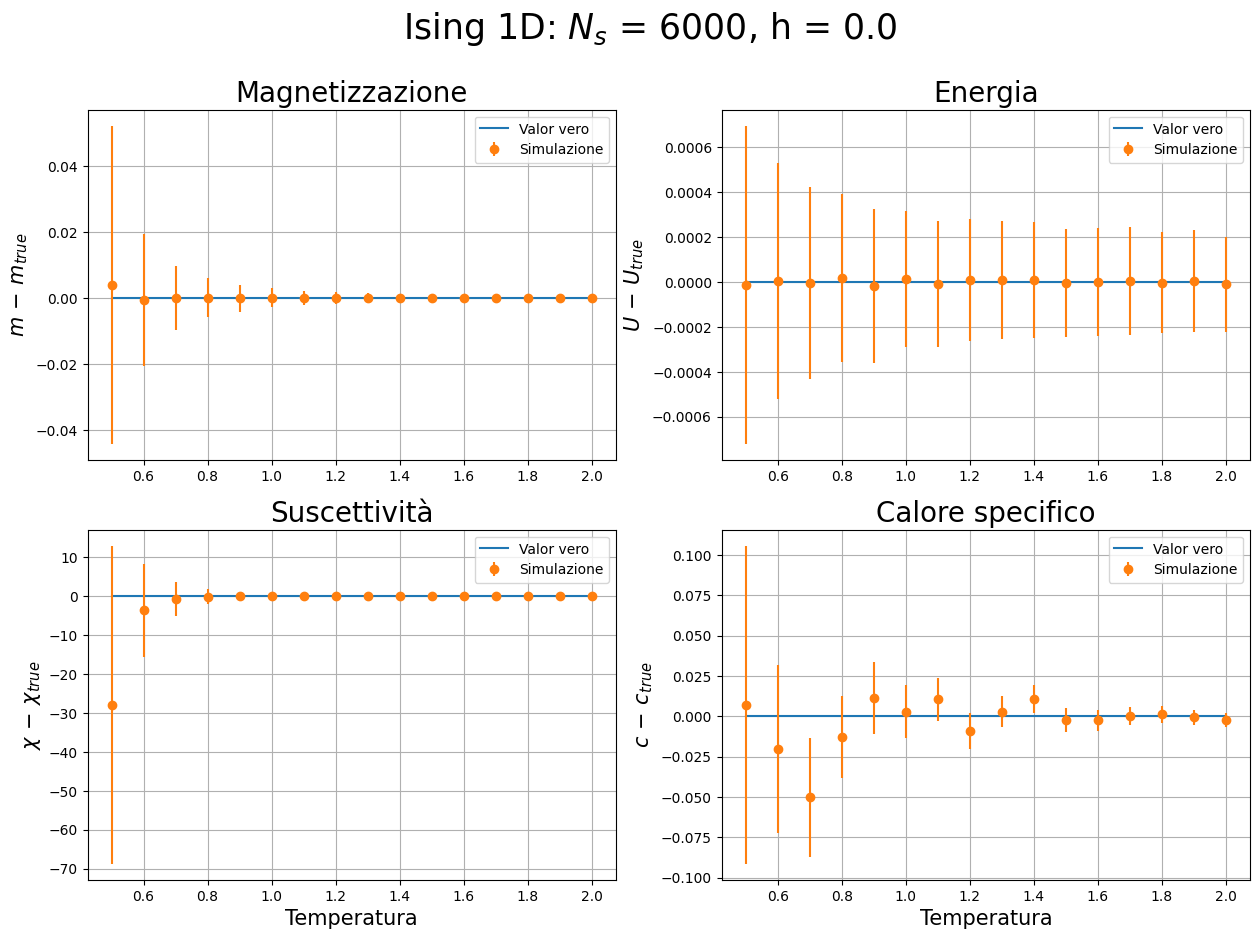
\includegraphics[width=0.65\textwidth]{Immagini/backupIsing1D/obs_6000_0.0_diff.png}

\end{frame}



%----------------------------------------%
%		       Nona slide	     	     %
%	     Osservabili per N = 1000   	 %
%----------------------------------------%
\begin{frame}
    \frametitle{Osservabili per $N_s$ = 1000, h = 0.02}
    \framesubtitle{}

    \centering
    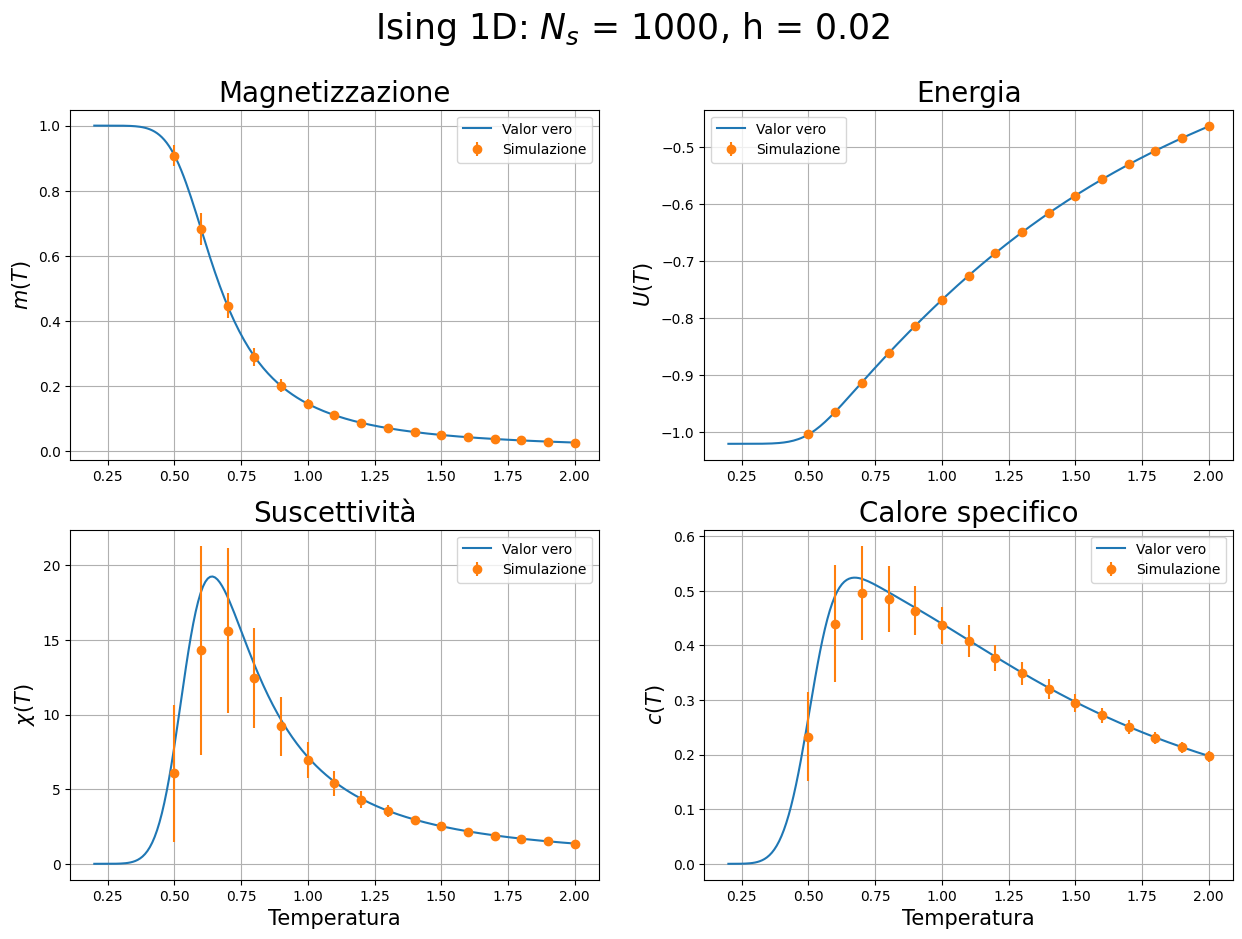
\includegraphics[width=0.65\textwidth]{Immagini/backupIsing1D/obs_1000_0.02.png}

\end{frame}



%----------------------------------------%
%		      Decima slide	     	     %
% Differenza dal valor vero per N = 1000 %
%----------------------------------------%
\begin{frame}
    \frametitle{Differenza dal valor vero per $N_s$ = 1000, h = 0.02}
    \framesubtitle{}

    \centering
    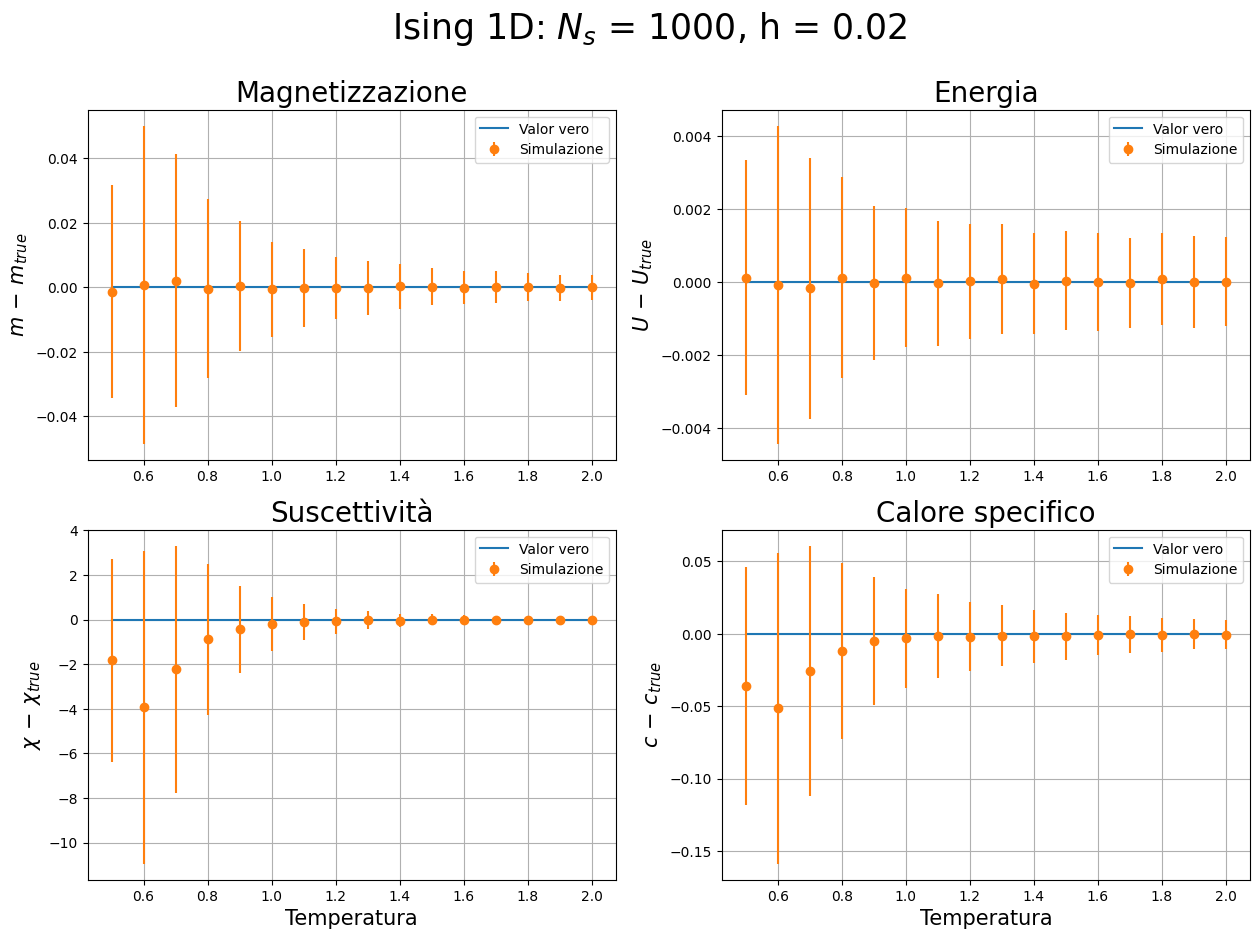
\includegraphics[width=0.65\textwidth]{Immagini/backupIsing1D/obs_1000_0.02_diff.png}

\end{frame}



%----------------------------------------%
%		     Undicesima slide	     	 %
%	     Osservabili per N = 3000   	 %
%----------------------------------------%
\begin{frame}
    \frametitle{Osservabili per $N_s$ = 3000, h = 0.02}
    \framesubtitle{}

    \centering
    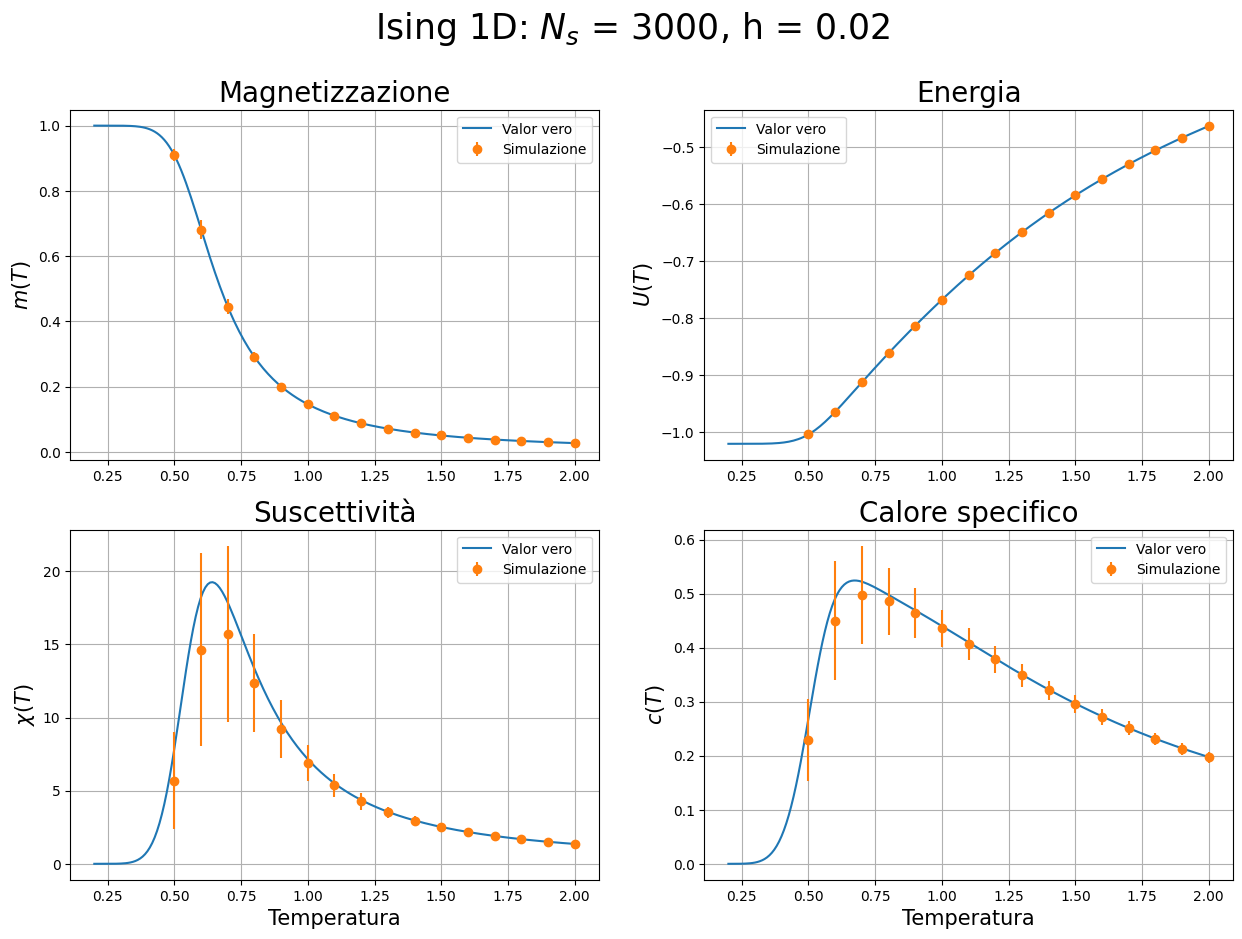
\includegraphics[width=0.65\textwidth]{Immagini/backupIsing1D/obs_3000_0.02.png}

\end{frame}



%----------------------------------------%
%		    Dodicesima slide    	     %
% Differenza dal valor vero per N = 3000 %
%----------------------------------------%
\begin{frame}
    \frametitle{Differenza dal valor vero per $N_s$ = 3000, h = 0.02}
    \framesubtitle{}

    \centering
    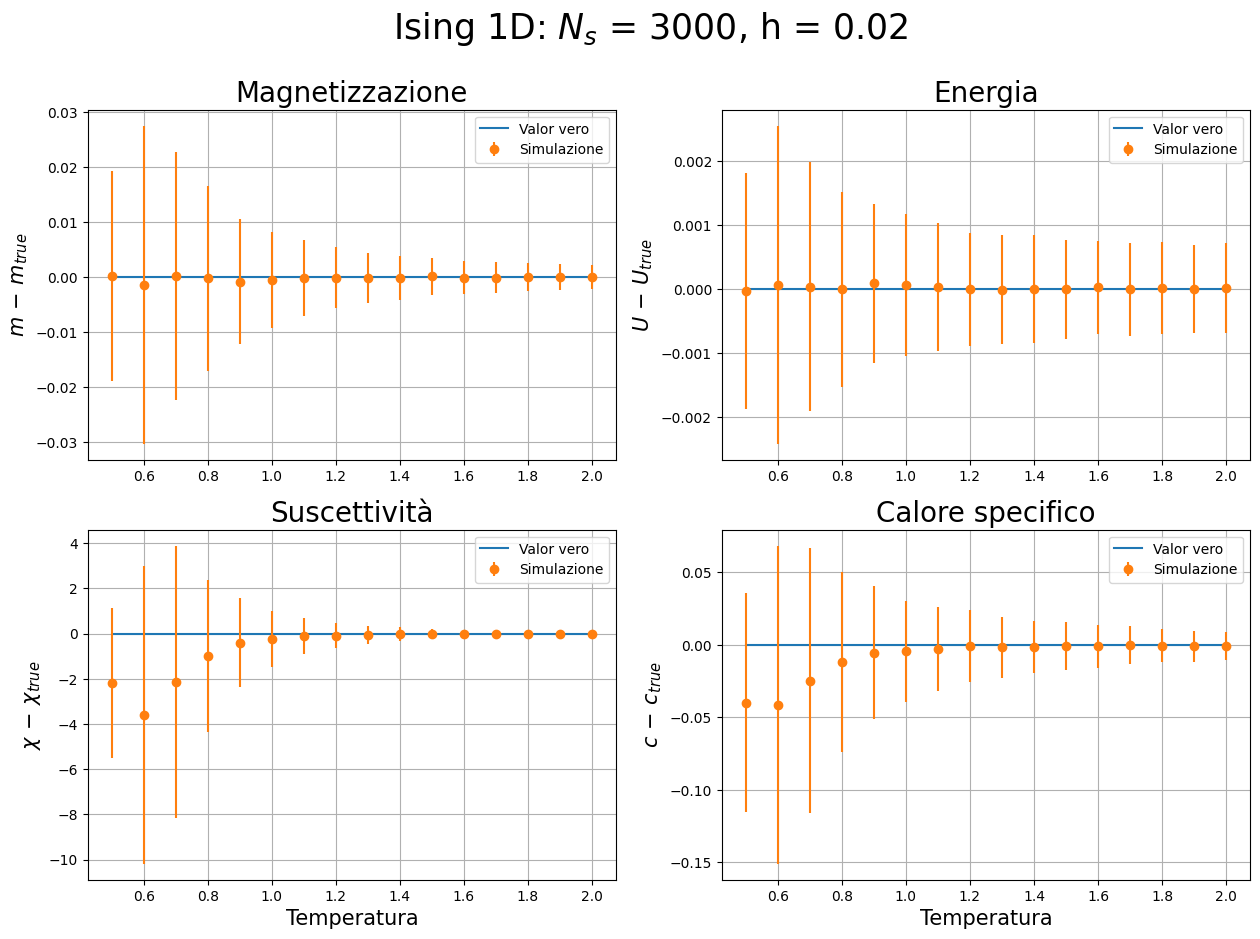
\includegraphics[width=0.65\textwidth]{Immagini/backupIsing1D/obs_3000_0.02_diff.png}

\end{frame}



%----------------------------------------%
%		     Tredicesima slide	         %
%	     Osservabili per N = 6000   	 %
%----------------------------------------%
\begin{frame}
    \frametitle{Osservabili per $N_s$ = 6000, h = 0.02}
    \framesubtitle{}

    \centering
    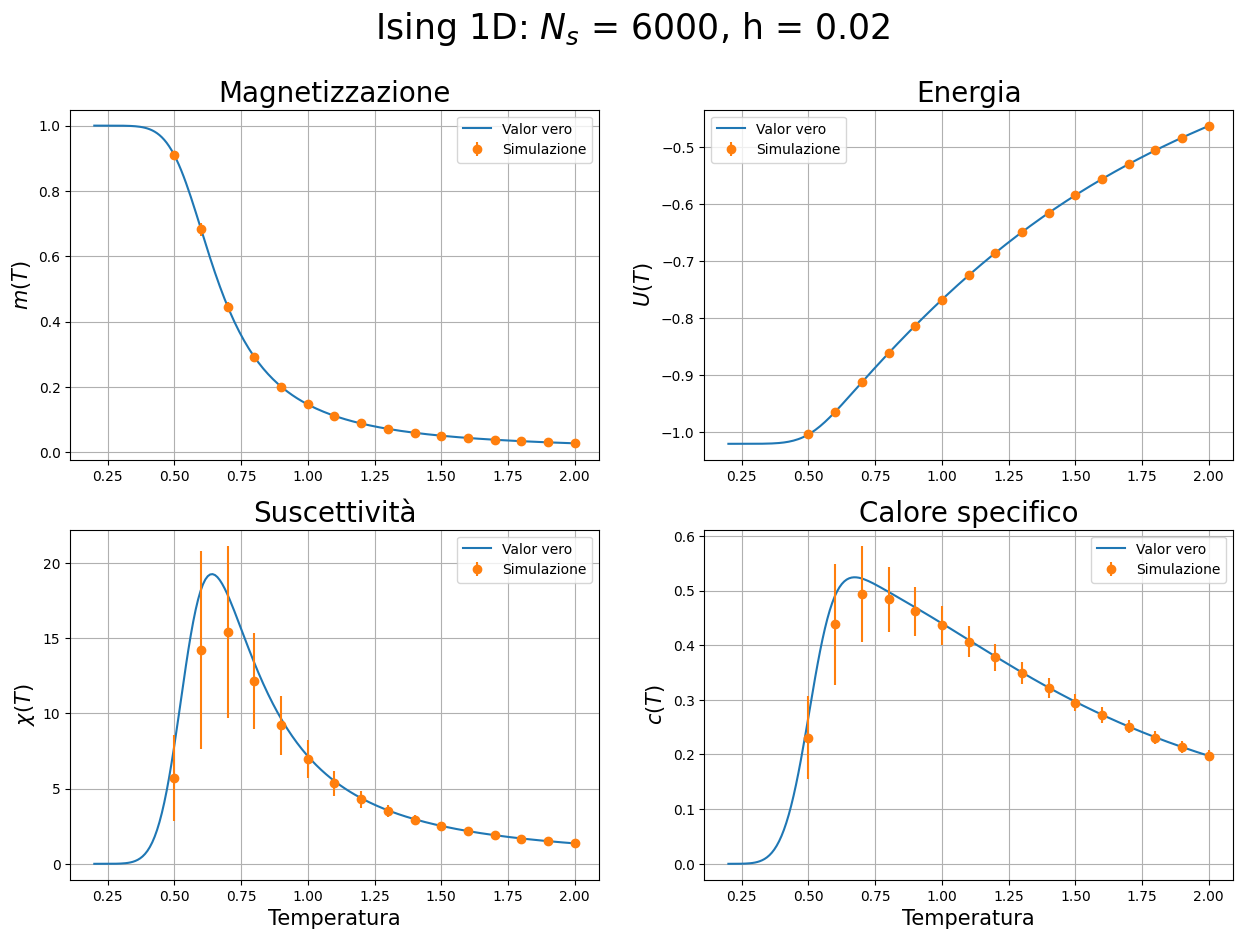
\includegraphics[width=0.65\textwidth]{Immagini/backupIsing1D/obs_6000_0.02.png}

\end{frame}



%----------------------------------------%
%		  Quattordicesima slide	     	 %
% Differenza dal valor vero per N = 6000 %
%----------------------------------------%
\begin{frame}
    \frametitle{Differenza dal valor vero per $N_s$ = 6000, h = 0.02}
    \framesubtitle{}

    \centering
    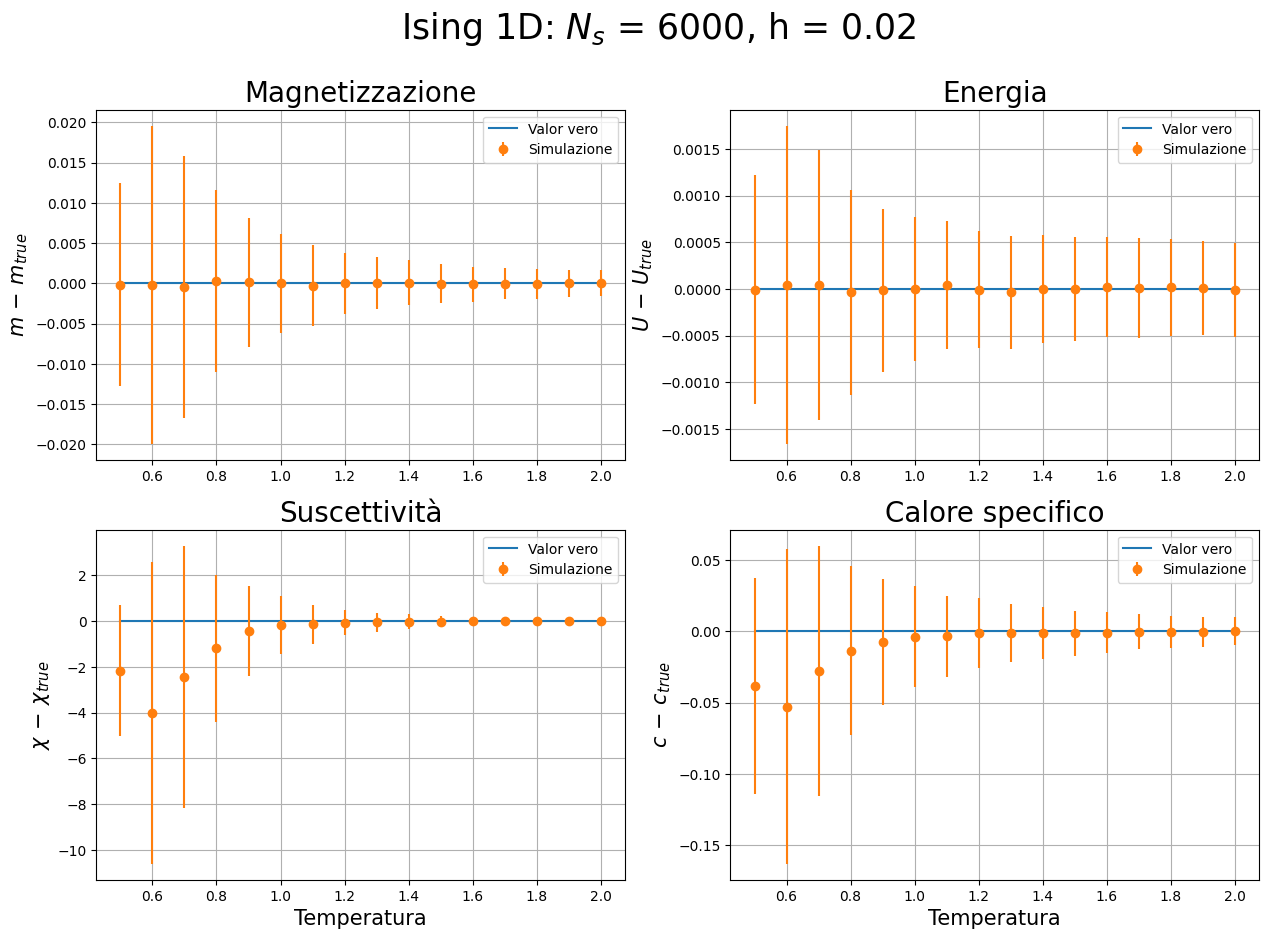
\includegraphics[width=0.65\textwidth]{Immagini/backupIsing1D/obs_6000_0.02_diff.png}

\end{frame}



%----------------------------------------%
%		     Quindicesima slide	     	 %
%	     Osservabili per N = 10000   	 %
%----------------------------------------%
\begin{frame}
    \frametitle{Osservabili per $N_s$ = 10000, h = 0.02}
    \framesubtitle{}

    \centering
    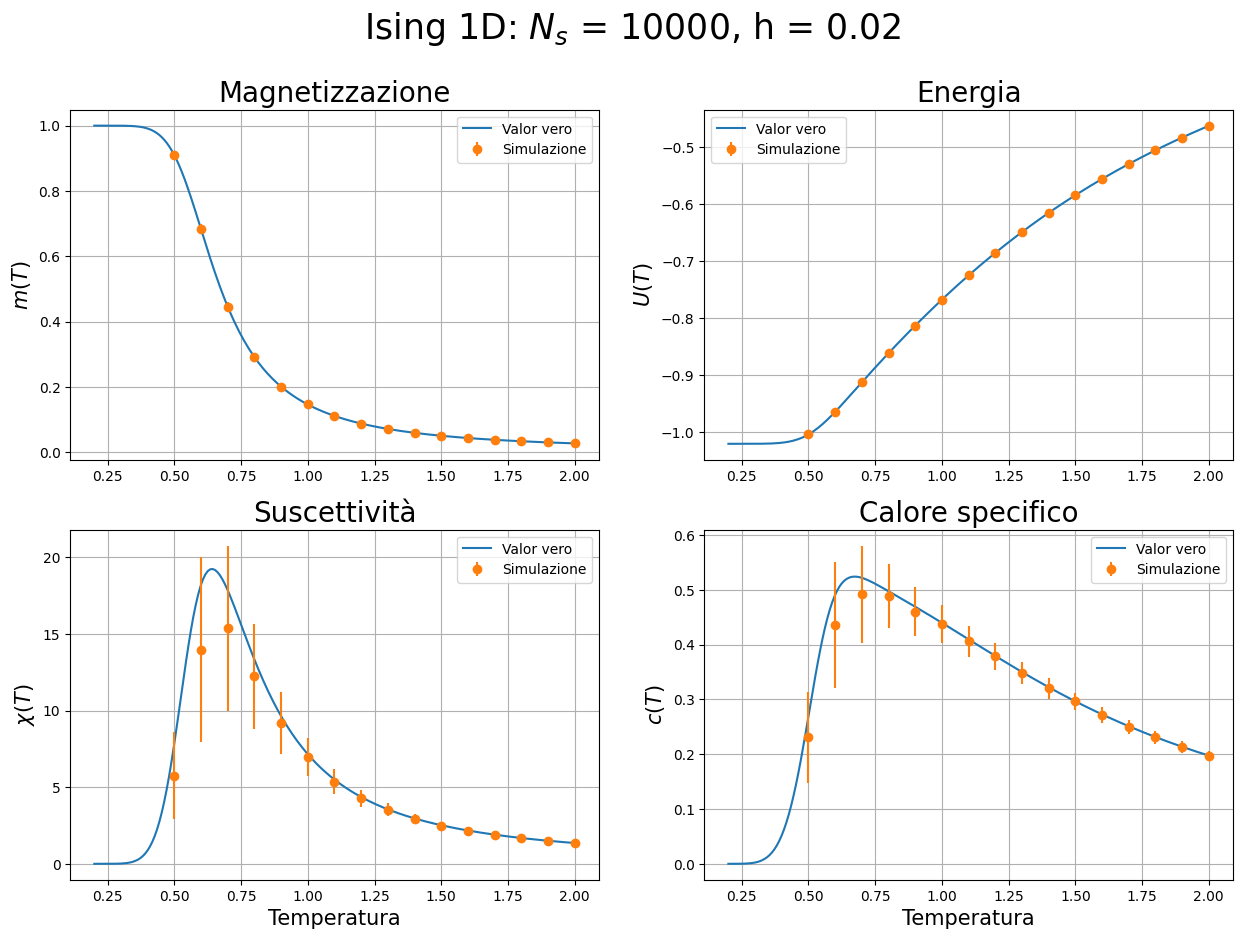
\includegraphics[width=0.65\textwidth]{Immagini/backupIsing1D/obs_10000_0.02.png}

\end{frame}



%----------------------------------------%
%		     Sedicesima slide	     	 %
%  Differenza dal valor vero, N = 10000  %
%----------------------------------------%
\begin{frame}
    \frametitle{Differenza dal valor vero per $N_s$ = 10000, h = 0.02}
    \framesubtitle{}

    \centering
    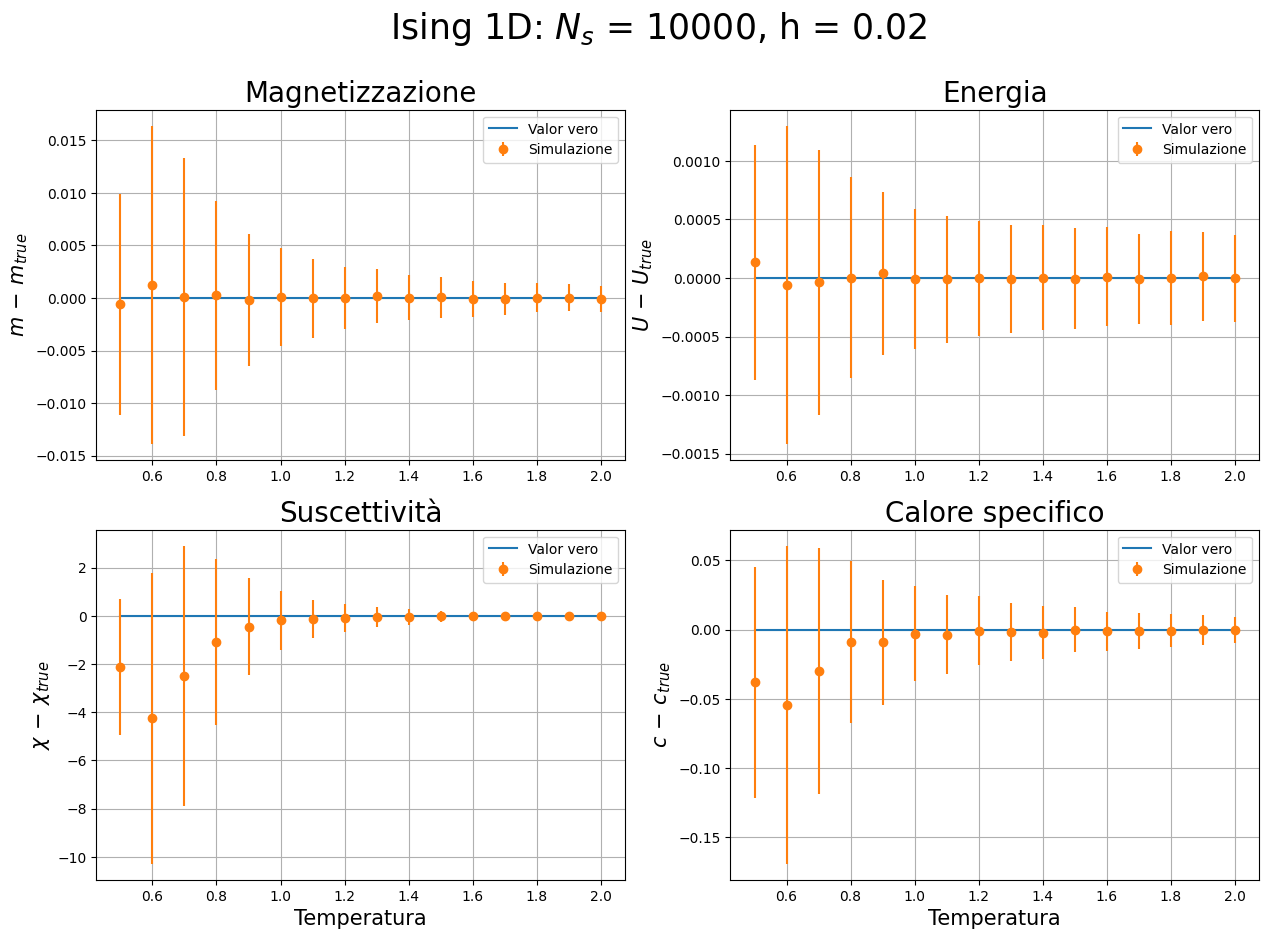
\includegraphics[width=0.65\textwidth]{Immagini/backupIsing1D/obs_10000_0.02_diff.png}

\end{frame}
